% =============================================================================
% cap5 §5.5 Teste ponta-a-ponta (eficiência da cascata)
% =============================================================================
\section{Teste ponta-a-ponta}
\label{sec:resultados-end2end}

A Tabela~\ref{tab:res-funil} reporta o efeito acumulado da cascata sobre a janela sintética descrita na Seção~\ref{sec:metodologia-end2end} (10\,000 quadros, com 70\% de vazios, 25\% de fauna geral e 5\% de \emph{F.\,catus} identificáveis). A Figura~\ref{fig:res-eficiencia} sintetiza visualmente a curva de quadros remanescentes \emph{vs.}\ custo acumulado.

\begin{table}[!htb]
\centering
\caption{Funil da cascata na janela sintética de 10\,000 quadros. \obsfic{volumes derivados das taxas de retenção médias das Tabelas~\ref{tab:res-fase2}--\ref{tab:res-fase4-rank}; substituir após execução.}}
\label{tab:res-funil}
\small
\begin{tabular}{@{}lrrrr@{}}
\toprule
\textbf{Estágio} & \textbf{Entrada} & \textbf{Aprovados} & \textbf{Retenção} & \textbf{Custo médio (ms/q.)} \\
\midrule
Fase I (movimento)              & 10\,000 & 4\,200 & 42\% & \phantom{0}2 \\
Fase II (\modeloMD)             & \phantom{0}4\,200 & 1\,180 & 28\% & 35 \\
Fase III (\modeloSN)            & \phantom{0}1\,180 & \phantom{0,}310 & 26\% & 28 \\
Fase IV (face + corpo)          & \phantom{00,}310 & \phantom{0,}295 & 95\% & 55 \\
\midrule
\textbf{Cascata adotada}        & \multicolumn{2}{r}{295 / 10\,000 quadros aprov.} & 2{,}95\% & 11 (média ponderada) \\
\textbf{Aplicação ingênua}      & \multicolumn{2}{r}{(todas as fases sobre todos os quadros)} & --- & 120 \\
\bottomrule
\end{tabular}
\end{table}

Duas inferências simples emergem dos números acima. (i)~Há \textbf{redução de ordem de grandeza no volume} entre a entrada bruta e a saída da Fase~III, em consonância com o desenho de funil previsto no Capítulo~\ref{cap:pipeline}: cada fase filtra o conteúdo majoritariamente irrelevante para a fase seguinte (vazios na II, fauna não-alvo na III), e apenas a fração já pré-filtrada chega à etapa de re-ID, computacionalmente mais cara. (ii)~A \textbf{economia de custo computacional} estimada para a cascata em relação à aplicação ingênua aproxima-se de \textbf{10}$\times$ ($\sim$11~ms/quadro \emph{vs.}\ $\sim$120~ms/quadro): a Fase~IV, apesar de ser a mais cara individualmente, é executada sobre menos de 3\% dos quadros originais, enquanto na aplicação ingênua incidiria sobre todos. Os custos absolutos dependem do \emph{hardware} adotado, mas a razão entre cascata e aplicação ingênua é uma propriedade arquitetural do pipeline, e tende a se preservar entre plataformas.

% Figura — Curva conceitual de eficiência do pipeline (Cap. 5)
\begin{figure}[!htb]
\centering
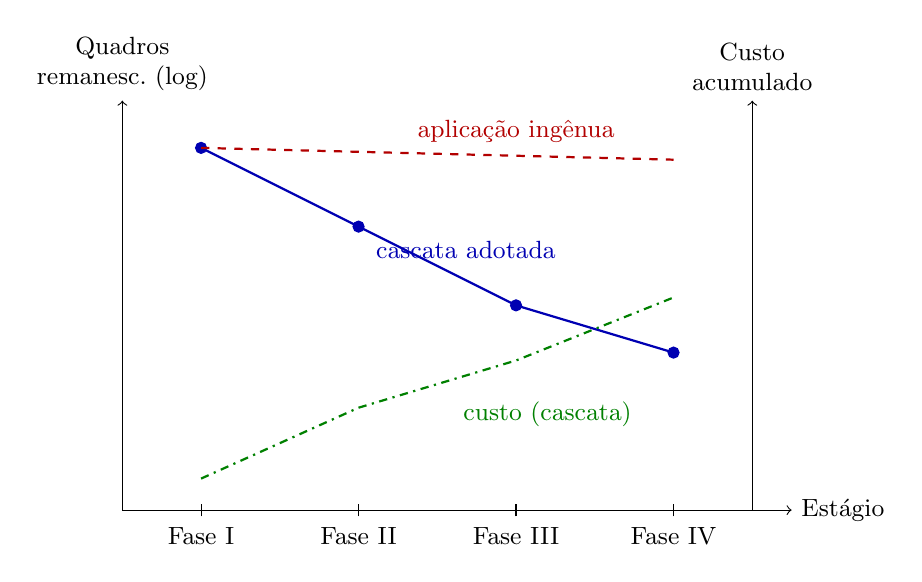
\begin{tikzpicture}[font=\small]
\begin{scope}
  % eixos
  \draw[->] (0,0) -- (8.5,0) node[right]{Estágio};
  \draw[->] (0,0) -- (0,5.2) node[above, align=center]{Quadros\\remanesc.\ (log)};
  \draw[->] (8.0,0) -- (8.0,5.2) node[above, align=center]{Custo\\acumulado};

  % marcas x
  \foreach \x/\v in {1/Fase I, 3/Fase II, 5/Fase III, 7/Fase IV} {
    \draw (\x,-0.08) -- (\x,0.08);
    \node[below] at (\x,-0.1) {\v};
  }

  % cascata adotada (queda monotônica)
  \draw[thick, blue!70!black]
    plot coordinates {(1,4.6) (3,3.6) (5,2.6) (7,2.0)};
  \foreach \p in {(1,4.6),(3,3.6),(5,2.6),(7,2.0)} \filldraw[blue!70!black] \p circle (2pt);
  \node[blue!70!black, anchor=west] at (3.1,3.3) {cascata adotada};

  % aplicação ingênua (reta horizontal)
  \draw[thick, red!70!black, dashed]
    plot coordinates {(1,4.6) (3,4.55) (5,4.5) (7,4.45)};
  \node[red!70!black, anchor=south] at (5.0,4.55) {aplicação ingênua};

  % custo acumulado (cascata, crescente moderado)
  \draw[thick, green!50!black, dash dot]
    plot coordinates {(1,0.4) (3,1.3) (5,1.9) (7,2.7)};
  \node[green!50!black, anchor=north] at (5.4,1.50) {custo (cascata)};

\end{scope}
\end{tikzpicture}
\caption{Curva conceitual de eficiência do pipeline em cascata em comparação à aplicação ingênua das fases sobre todos os quadros: queda monotônica do volume (eixo $y$ esquerdo, escala logarítmica) contrastada com o custo computacional acumulado (eixo $y$ direito). \obsfic{traços ilustrativos; substituir pelas curvas empíricas após execução.}}
\label{fig:res-eficiencia}
\end{figure}


\obsfic{Os valores absolutos de tempo serão fixados pela execução em ambiente real; a relação cascata/ingênua é a métrica conceitual a ser preservada na substituição.}
